\newpage
\begin{center}
\textbf{ГЛАВА 3}\\
\textbf{ДИФФУЗИЯ ОТ ТРОЙНОЙ ДО КРИТИЧЕСКОЙ ТОЧКИ}
\end{center}
\refstepcounter{chapter}


% \section*{}
\addcontentsline{toc}{chapter}{ГЛАВА 3. Диффузия от тройной до критической точки}
%\section{Расчет спектров в МД}

\section{Изучение диффузии методами молекулярной динамики}\label{C3_1}

Текст

\begin{figure}[htbp!]
\begin{center}
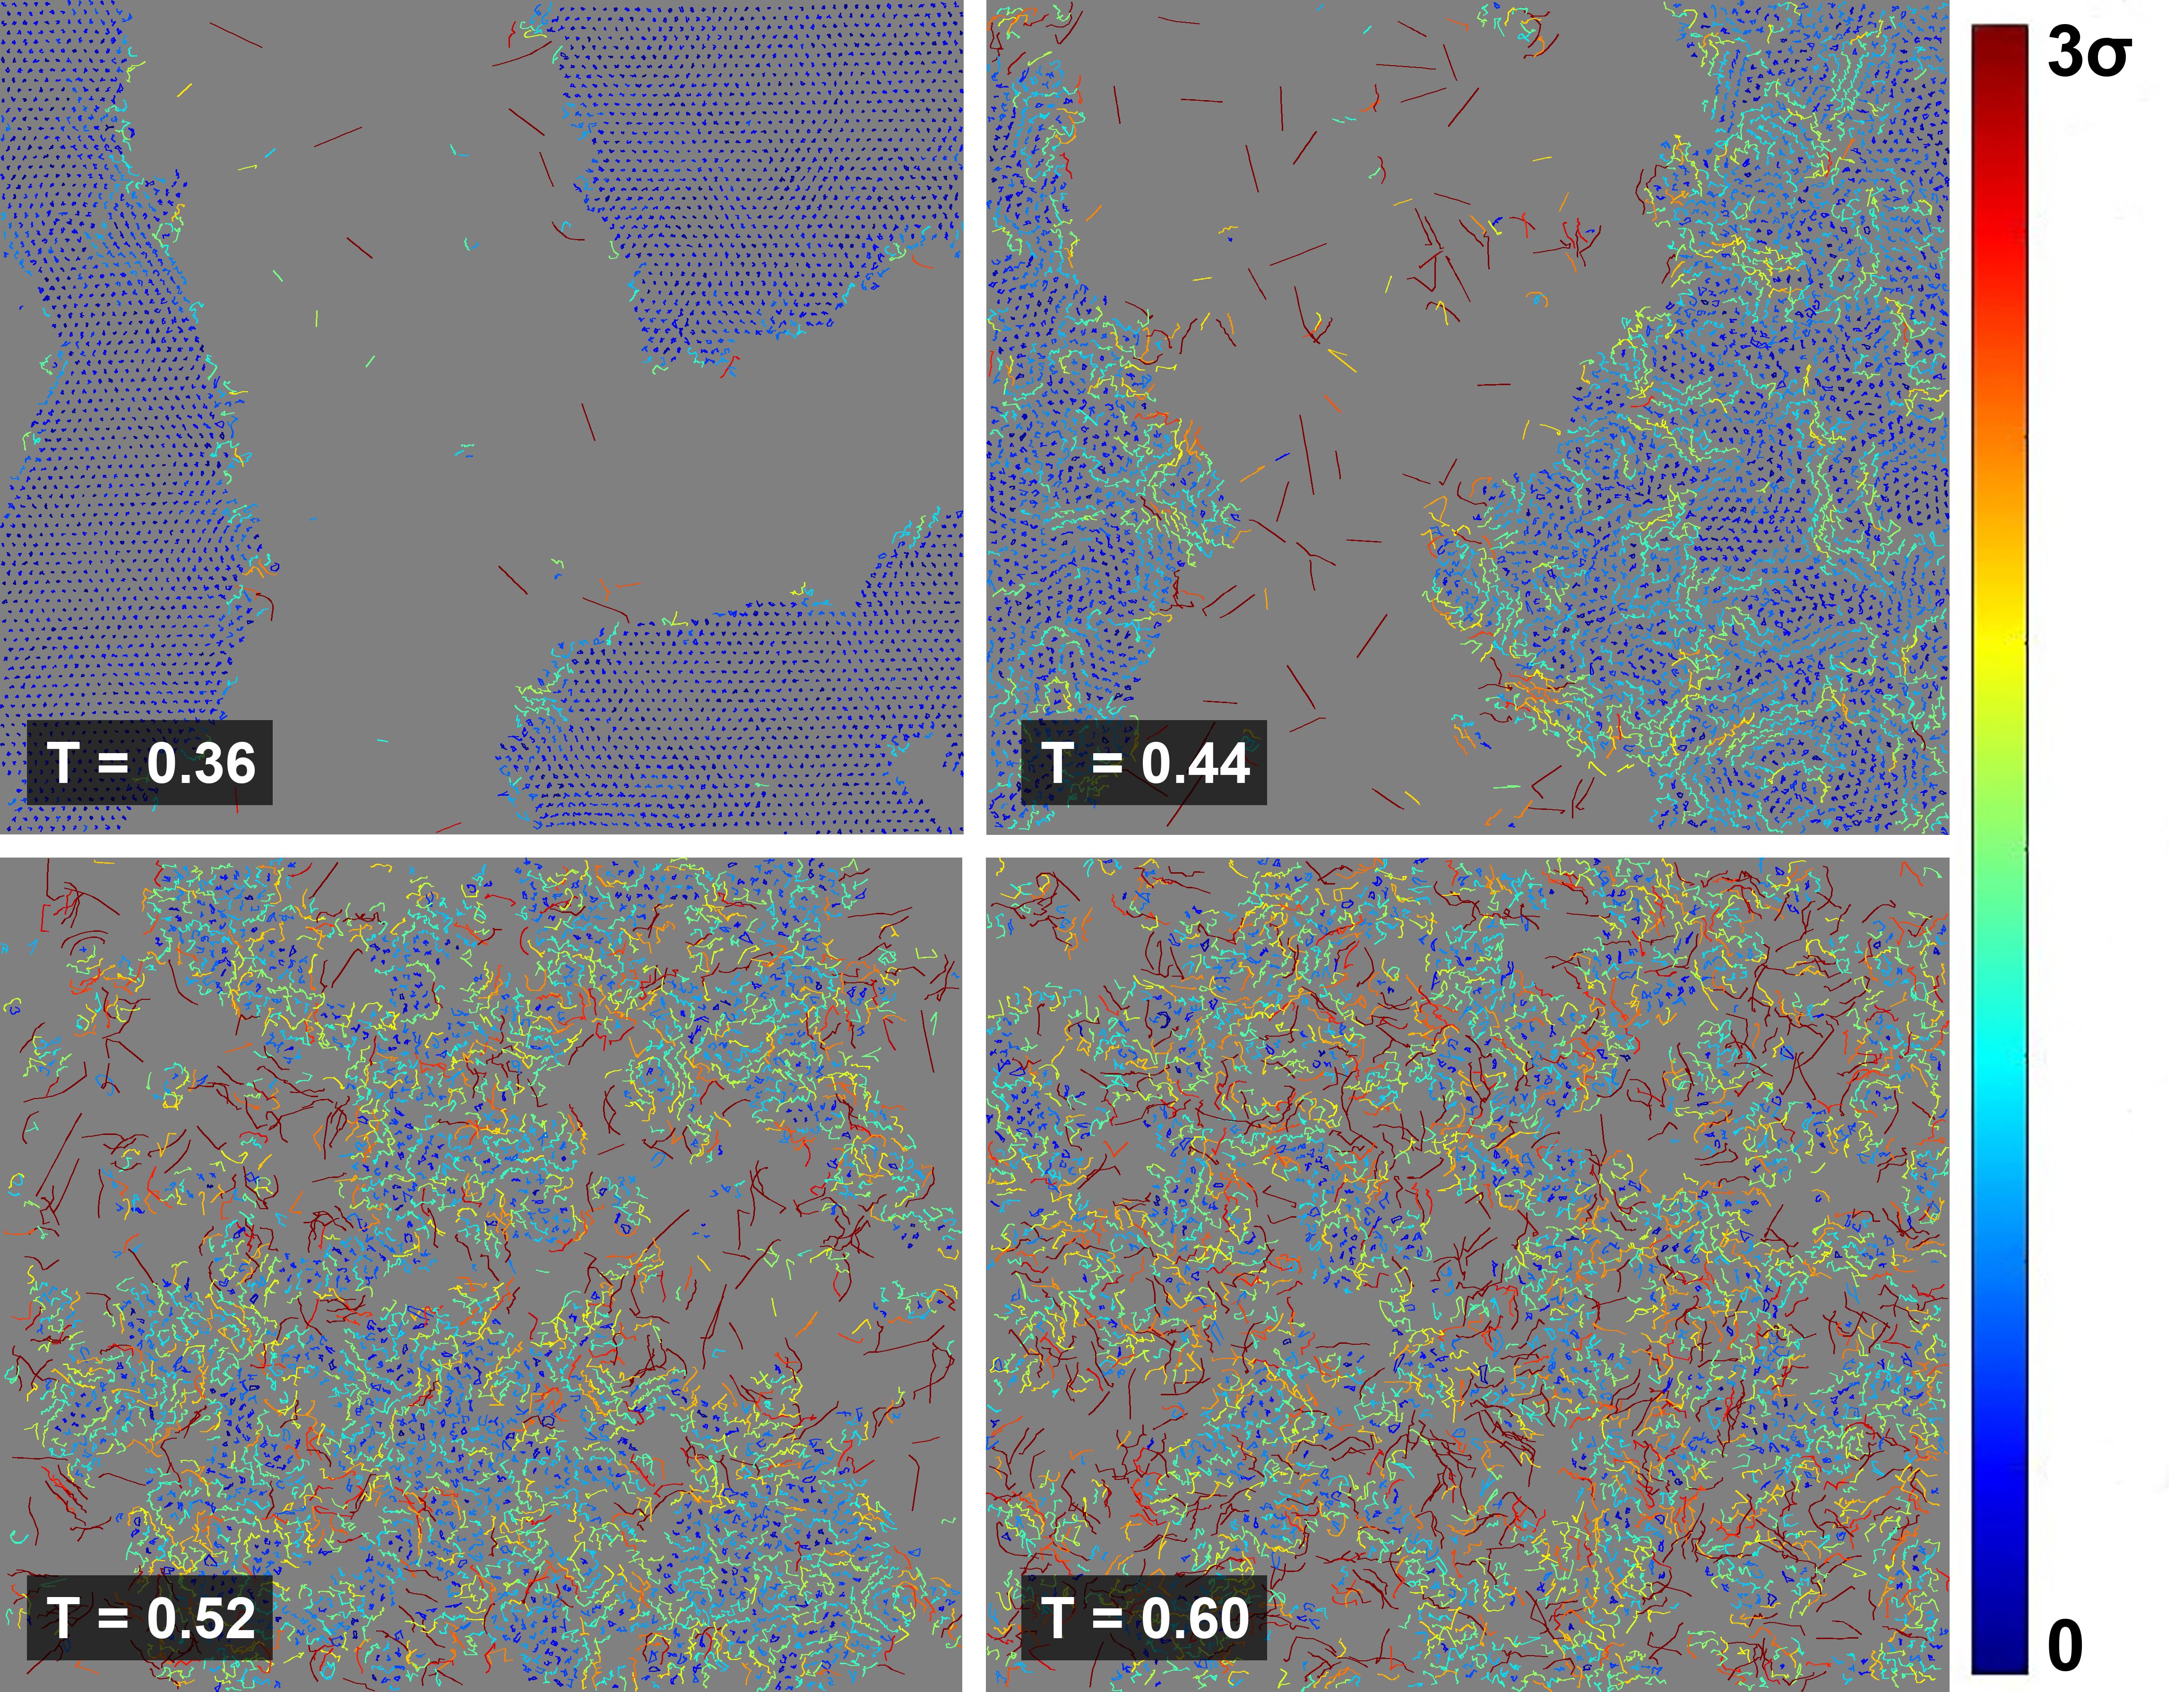
\includegraphics[width=0.7\textwidth]{Diffusion}
\caption{Смещение частиц от начального положения за 10 кадров моделирования. Цветом показана величина смещения в $\sigma$ (единица измерения длинны).}
\label{ris15}
\end{center}
\end{figure}


Текст

\begin{figure}[htbp!]
\begin{center}
\begin{minipage}[h]{0.45\linewidth}
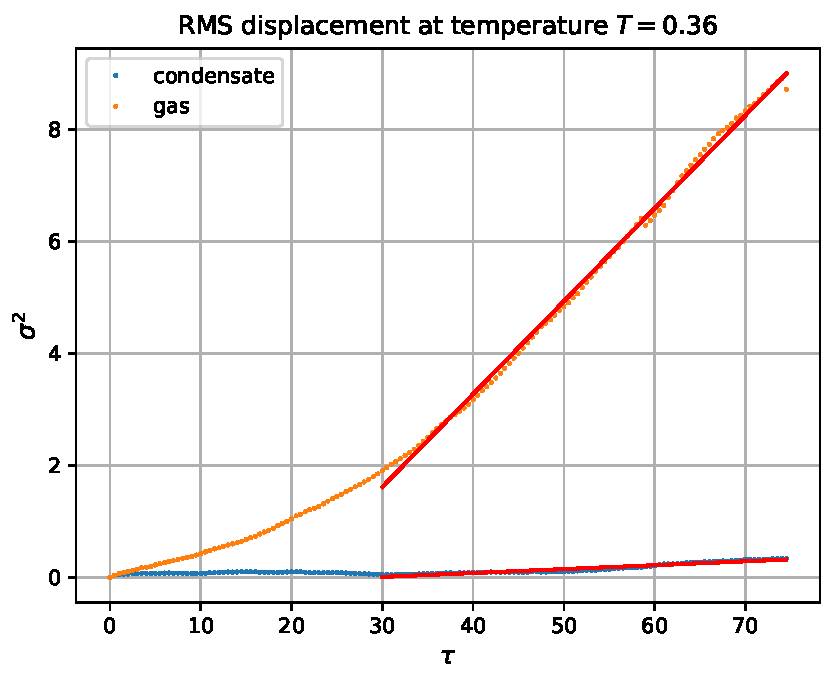
\includegraphics[width=\textwidth, keepaspectratio]{diffusion_fit_0.36}
\end{minipage}
%\hfill
\begin{minipage}[h]{0.45\linewidth}
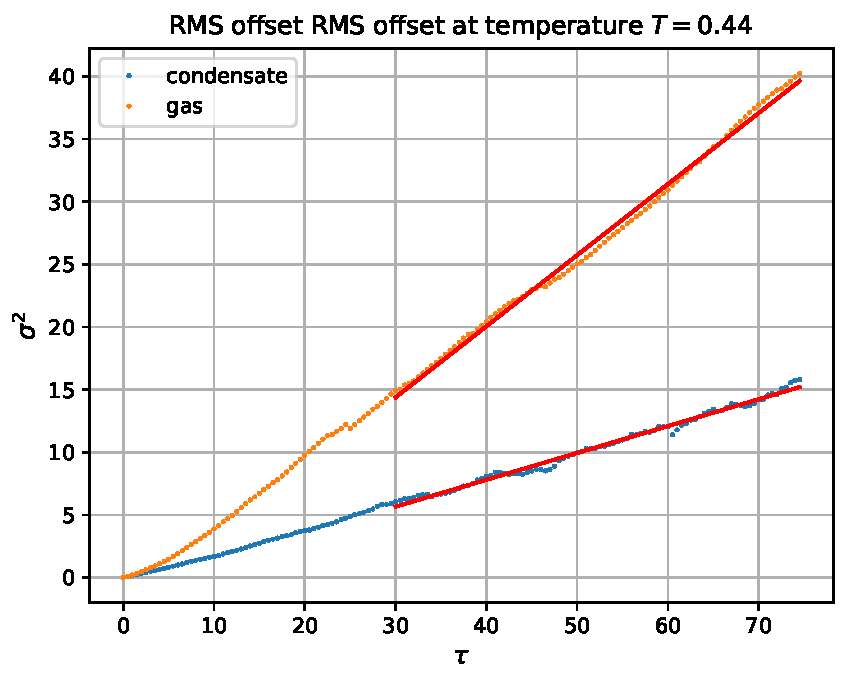
\includegraphics[width=\textwidth, keepaspectratio]{diffusion_fit_0.44}
\end{minipage}

%\vfill

\begin{minipage}[h]{0.45\linewidth}
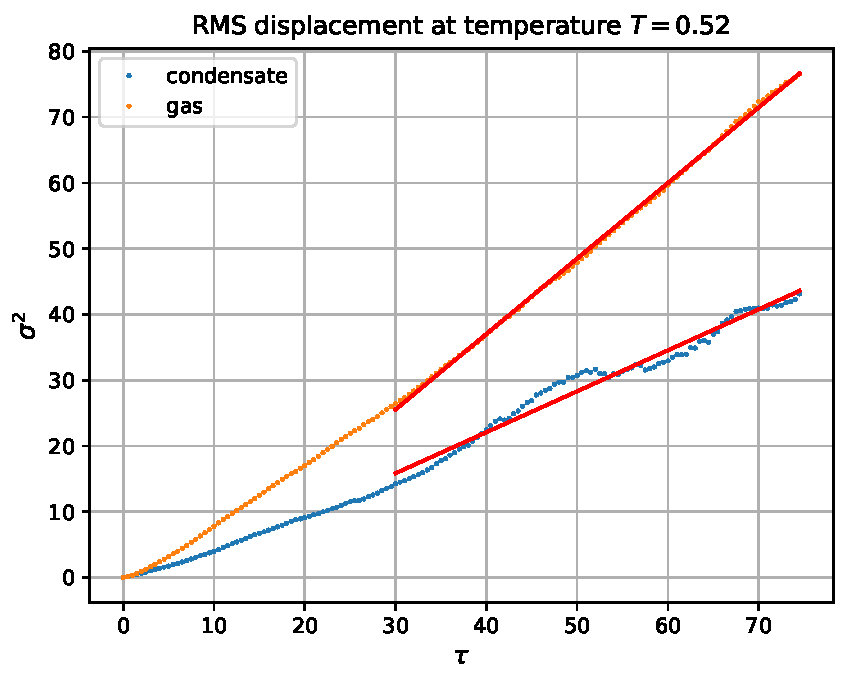
\includegraphics[width=\textwidth, keepaspectratio]{diffusion_fit_0.52}
\end{minipage}
%\hfill
\begin{minipage}[h]{0.45\linewidth}
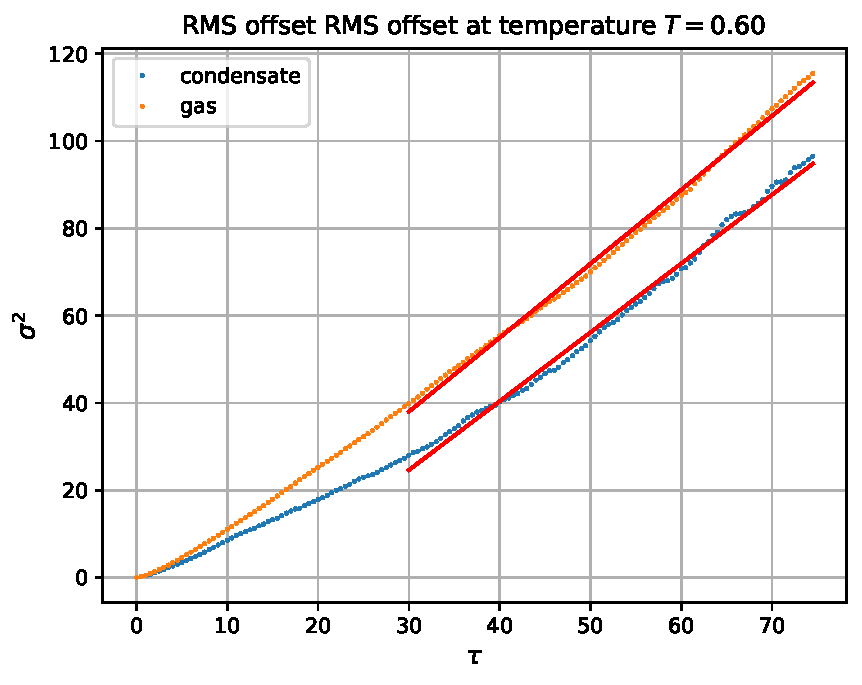
\includegraphics[width=\textwidth, keepaspectratio]{diffusion_fit_0.60}
\end{minipage}
\caption{Временная зависимость среднеквадратичного смещения частиц для различных температур на примере потенциала Леннарда-Джонса.}
\label{ris16}
\end{center}
\end{figure}

Текст

Текст

\begin{figure}[htbp!]
\begin{center}
\begin{minipage}[h]{0.45\linewidth}
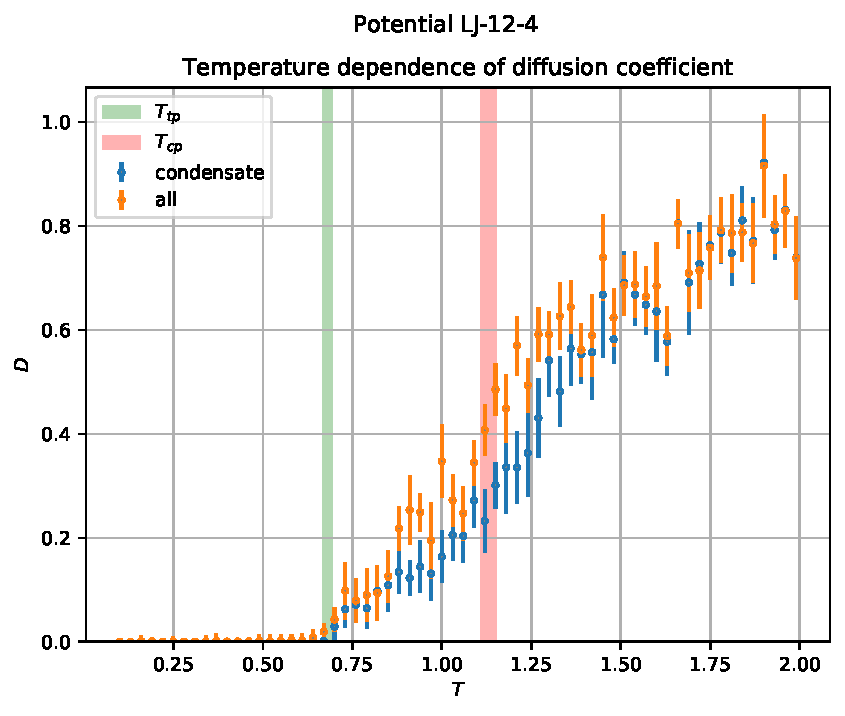
\includegraphics[width=\textwidth, keepaspectratio]{plot_diffusion_Potential LJ-12-4_1}
\end{minipage}
%\hfill
\begin{minipage}[h]{0.45\linewidth}
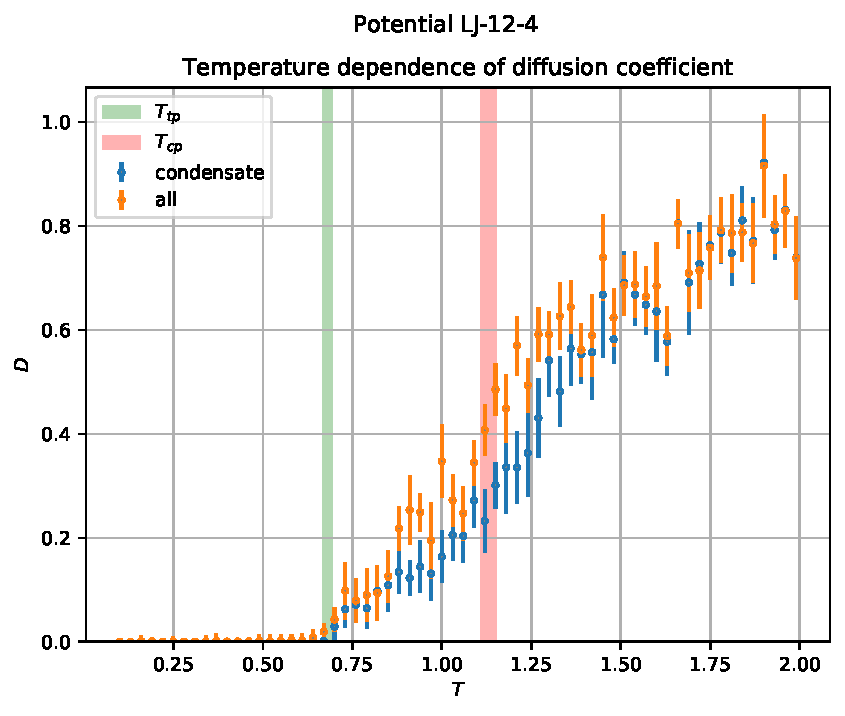
\includegraphics[width=\textwidth, keepaspectratio]{plot_diffusion_Potential LJ-12-4_1}
\end{minipage}

%\vfill

\begin{minipage}[h]{0.45\linewidth}
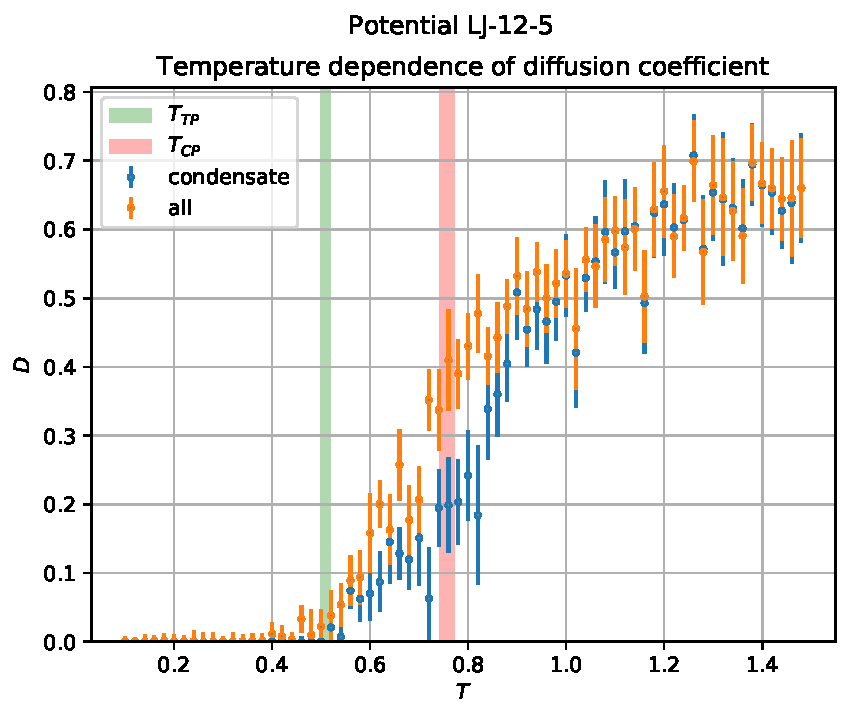
\includegraphics[width=\textwidth, keepaspectratio]{plot_diffusion_Potential LJ-12-5_1}
\end{minipage}
%\hfill
\begin{minipage}[h]{0.45\linewidth}
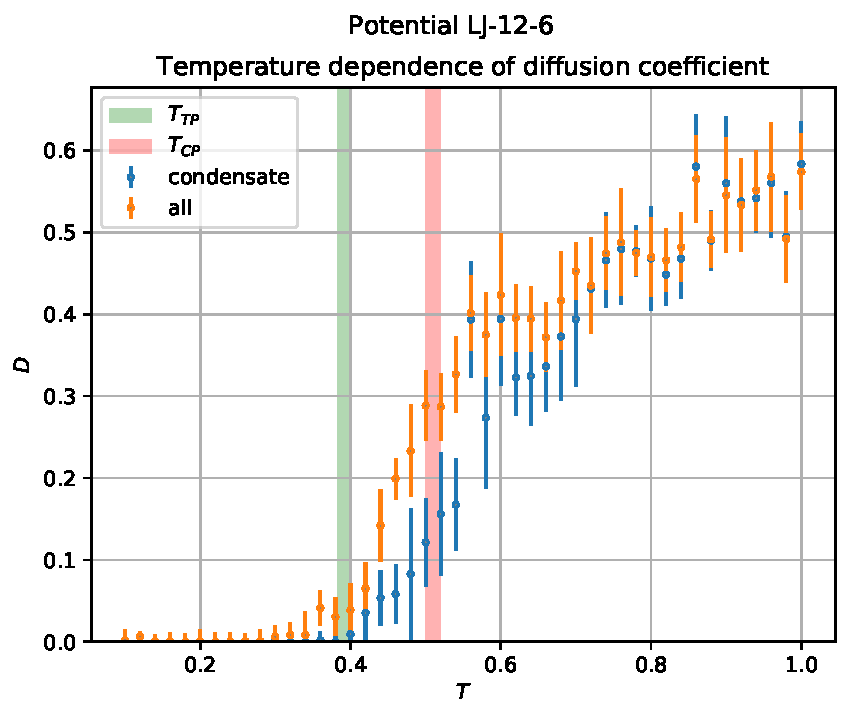
\includegraphics[width=\textwidth, keepaspectratio]{plot_diffusion_Potential LJ-12-6_1}
\end{minipage}
\caption{Температурная зависимость коэффициента диффузии для различных потенциалов взаимодействия. Не доделана!}
\label{ris17}
\end{center}
\end{figure}

Текст

Текст

\begin{figure}[htbp!]
\begin{center}
\begin{minipage}[h]{0.45\linewidth}
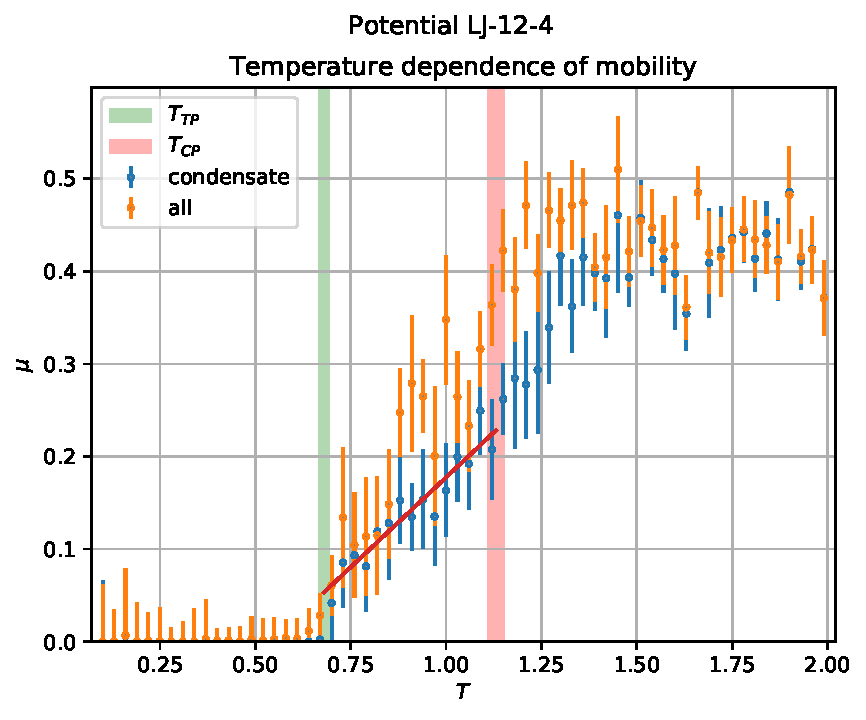
\includegraphics[width=\textwidth, keepaspectratio]{plot_mobility_Potential LJ-12-4_1}
\end{minipage}
%\hfill
\begin{minipage}[h]{0.45\linewidth}
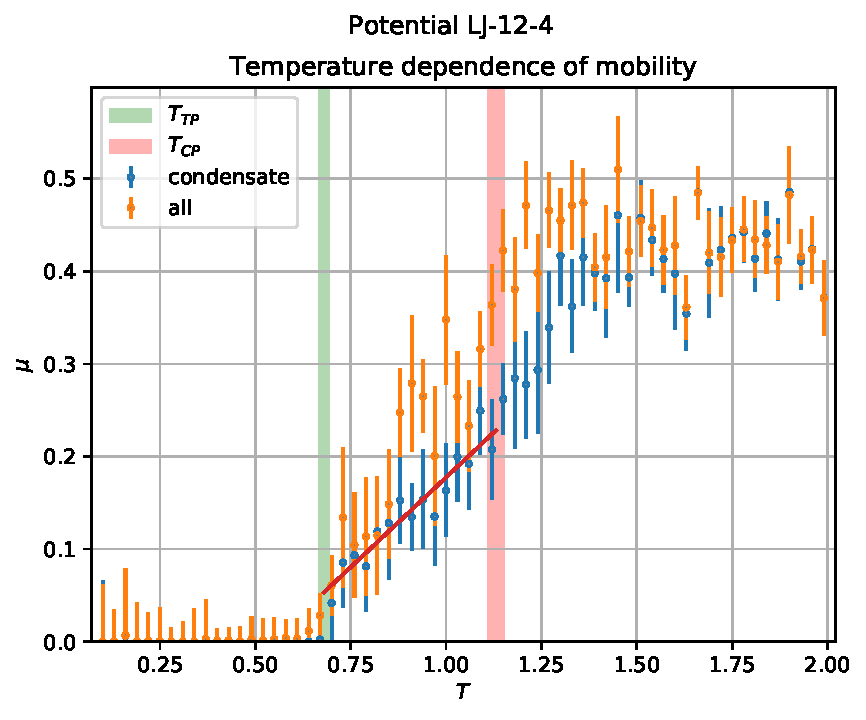
\includegraphics[width=\textwidth, keepaspectratio]{plot_mobility_Potential LJ-12-4_1}
\end{minipage}

%vfill

\begin{minipage}[h]{0.45\linewidth}
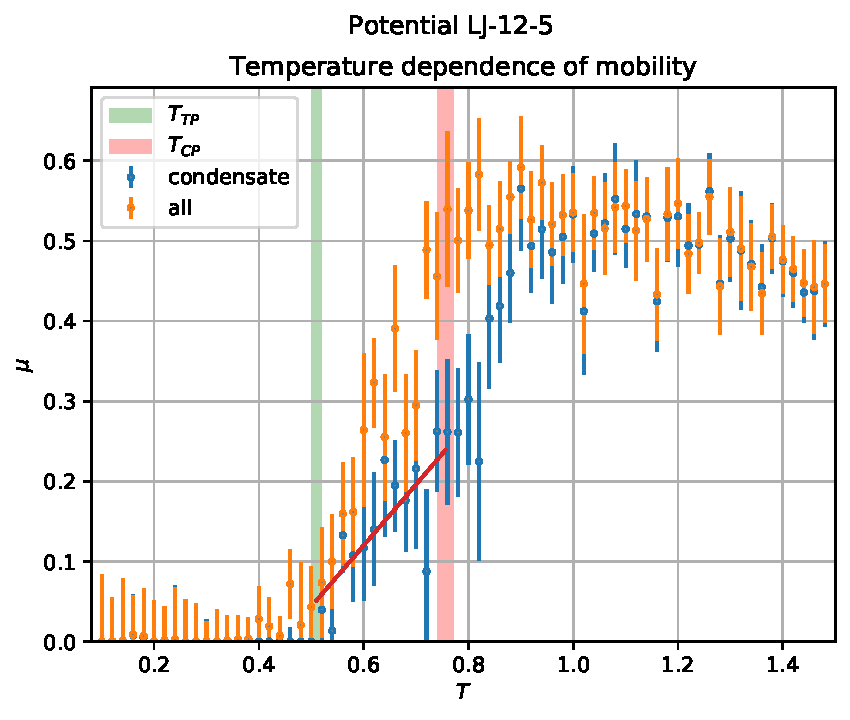
\includegraphics[width=\textwidth, keepaspectratio]{plot_mobility_Potential LJ-12-5_1}
\end{minipage}
%\hfill
\begin{minipage}[h]{0.45\linewidth}
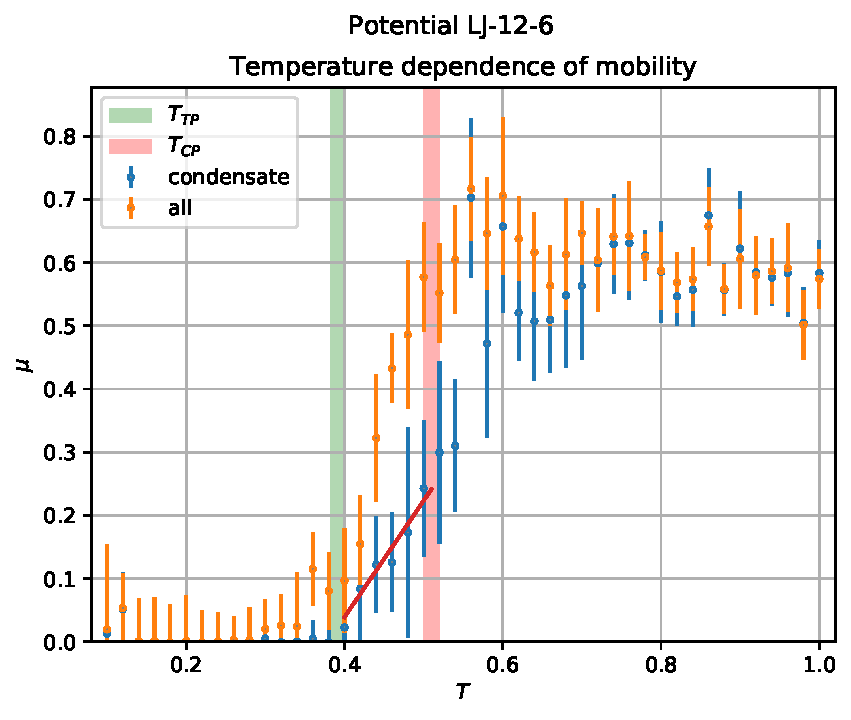
\includegraphics[width=\textwidth, keepaspectratio]{plot_mobility_Potential LJ-12-6_1}
\end{minipage}
\caption{Температурная зависимость мобильности для различных потенциалов взаимодействия. Не доделана!}
\label{ris18}
\end{center}
\end{figure}

Текст

Текст

\begin{figure}[htbp!]
\begin{center}
\begin{minipage}[h]{0.45\linewidth}
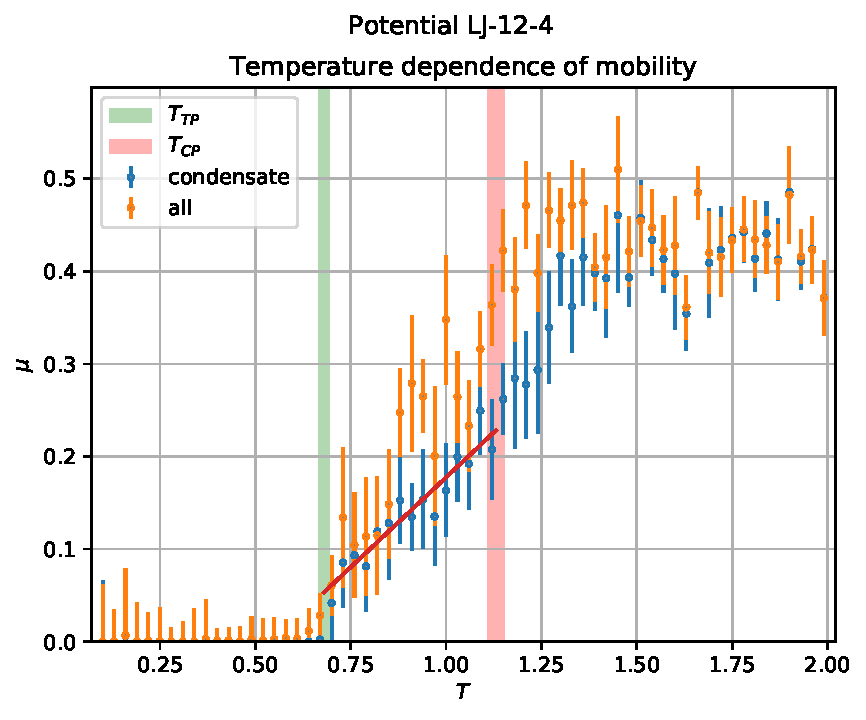
\includegraphics[width=\textwidth, keepaspectratio]{plot_mobility_Potential LJ-12-4_1}
\end{minipage}
%\hfill
\begin{minipage}[h]{0.45\linewidth}
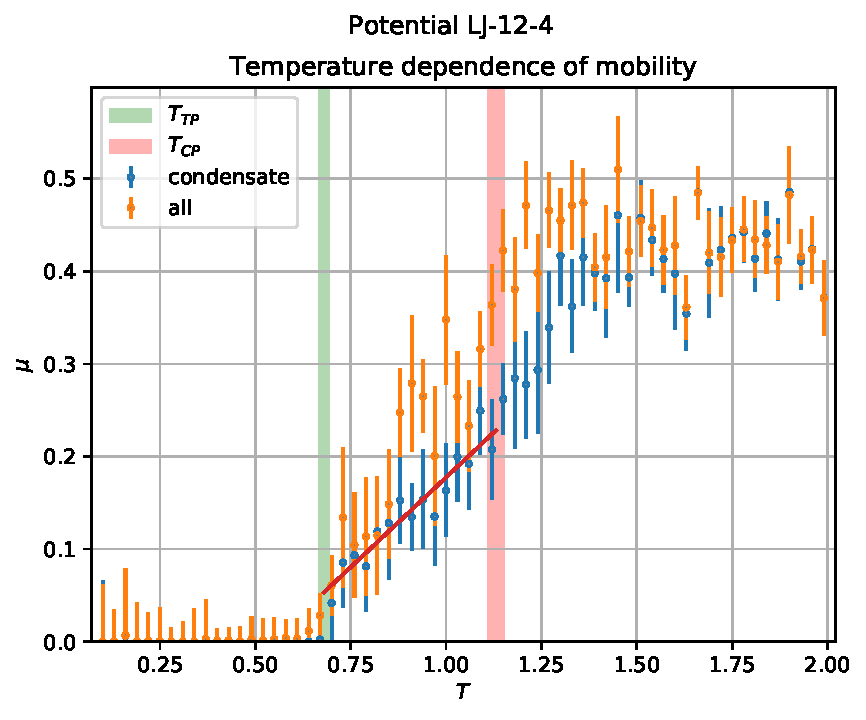
\includegraphics[width=\textwidth, keepaspectratio]{plot_mobility_Potential LJ-12-4_1}
\end{minipage}

%\vfill

\begin{minipage}[h]{0.45\linewidth}
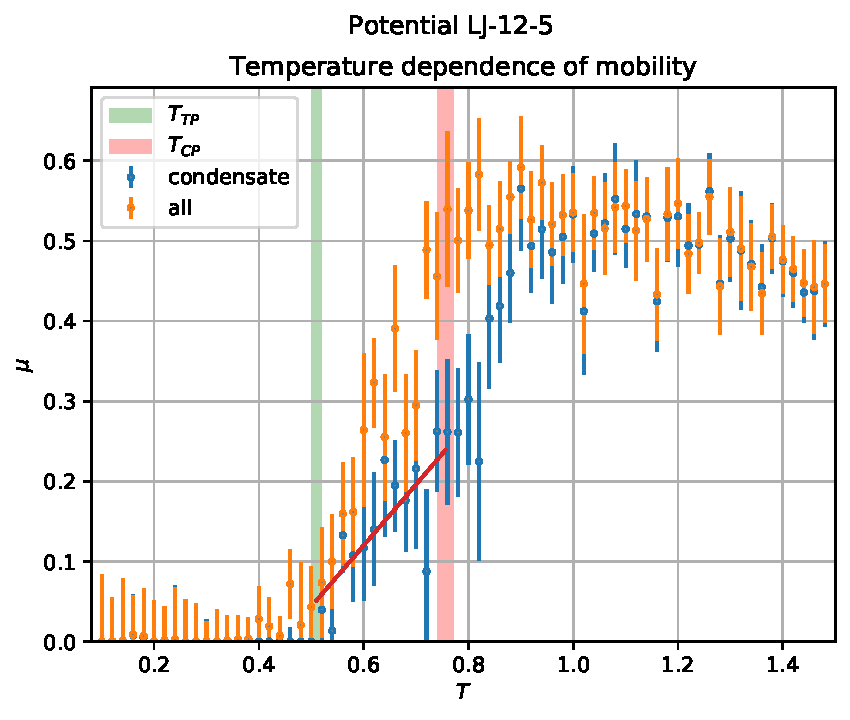
\includegraphics[width=\textwidth, keepaspectratio]{plot_mobility_Potential LJ-12-5_1}
\end{minipage}
%\hfill
\begin{minipage}[h]{0.45\linewidth}
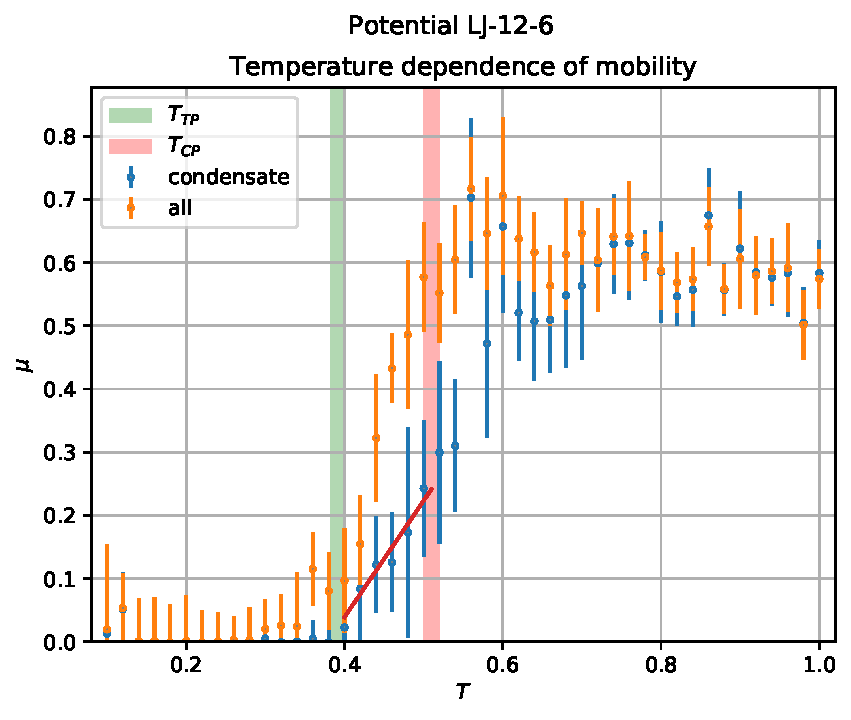
\includegraphics[width=\textwidth, keepaspectratio]{plot_mobility_Potential LJ-12-6_1}
\end{minipage}
\caption{Температурная зависимость мобильности для различных потенциалов взаимодействия. Не доделана!}
\label{ris19}
\end{center}
\end{figure}

Текст

\section{Связь термодинамических параметров, и параметров переноса вещества}\label{C3_2}

Текст

Текст

\begin{figure}[htbp!]
\begin{center}
\begin{minipage}[h]{0.45\linewidth}
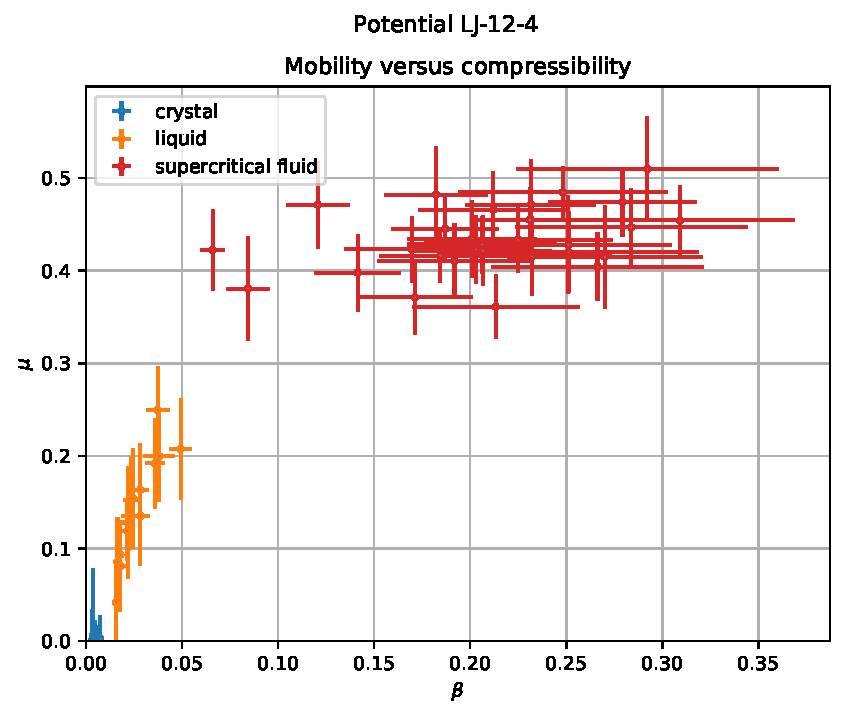
\includegraphics[width=\textwidth, keepaspectratio]{plot_compress_mobility_Potential LJ-12-4_1}
\end{minipage}
%\hfill
\begin{minipage}[h]{0.45\linewidth}
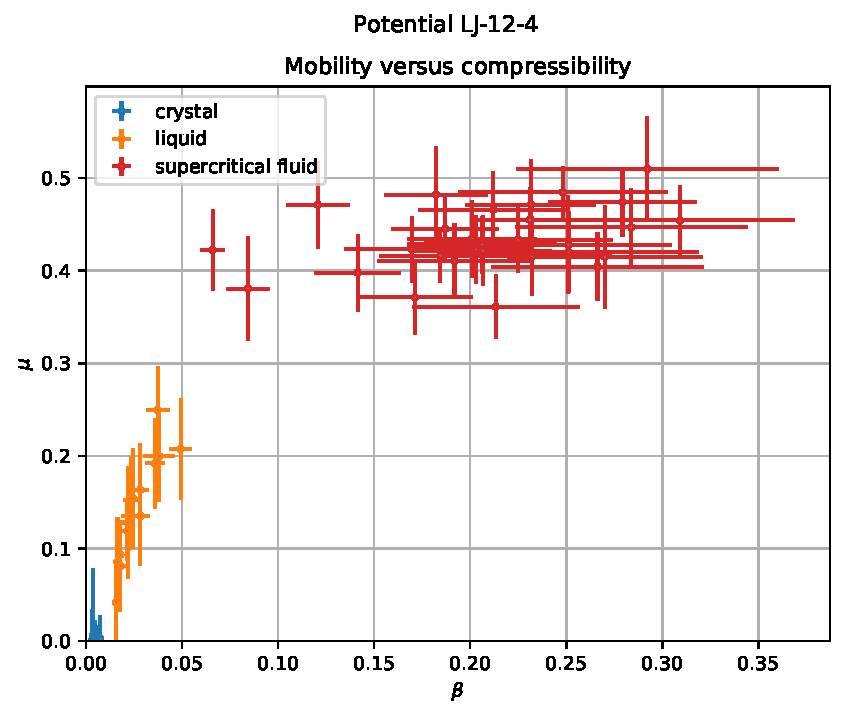
\includegraphics[width=\textwidth, keepaspectratio]{plot_compress_mobility_Potential LJ-12-4_1}
\end{minipage}

%\vfill

\begin{minipage}[h]{0.45\linewidth}
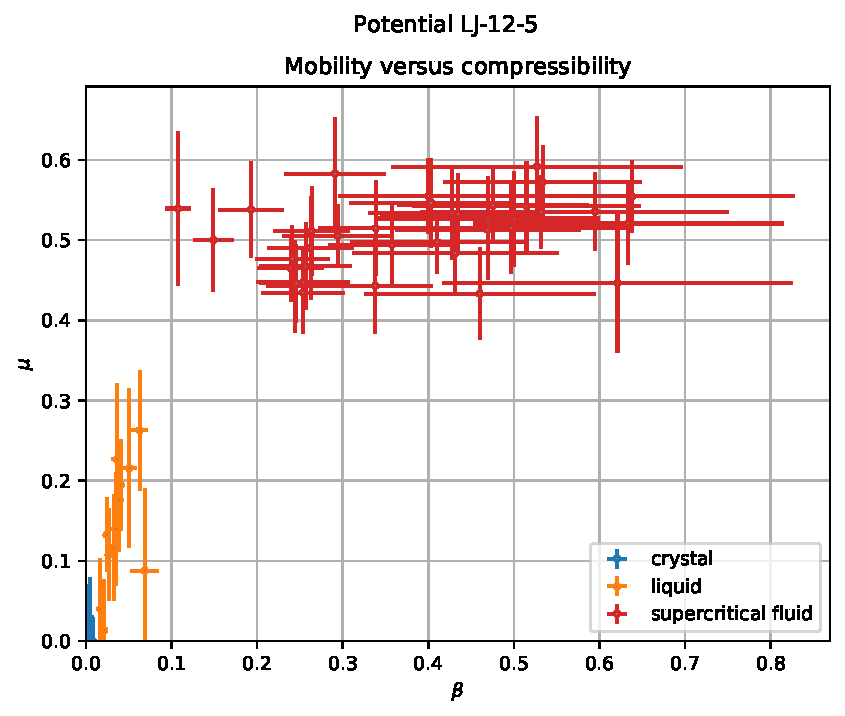
\includegraphics[width=\textwidth, keepaspectratio]{plot_compress_mobility_Potential LJ-12-5_1}
\end{minipage}
%\hfill
\begin{minipage}[h]{0.45\linewidth}
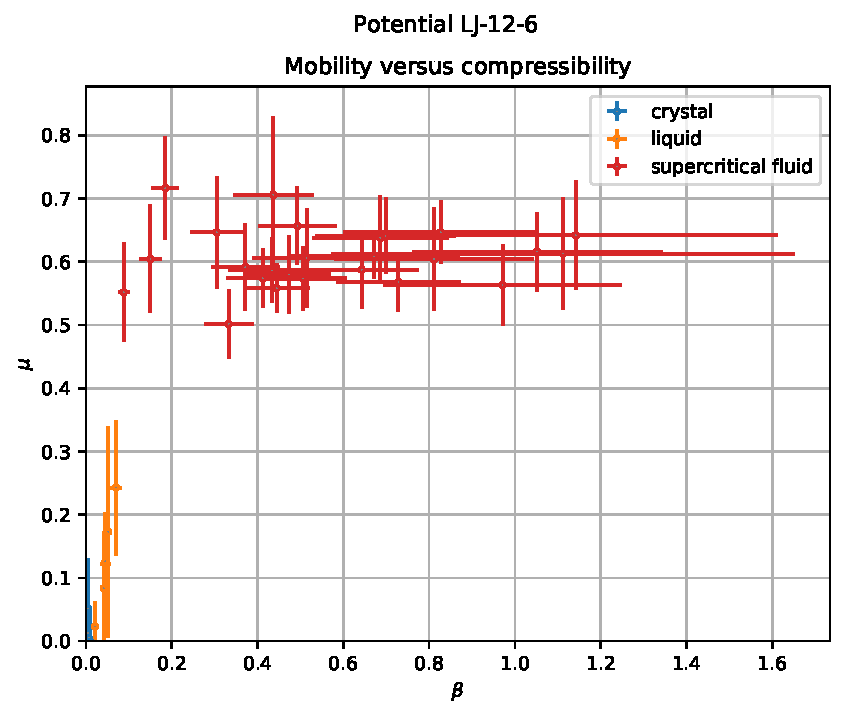
\includegraphics[width=\textwidth, keepaspectratio]{plot_compress_mobility_Potential LJ-12-6_1}
\end{minipage}
\caption{Зависимость мобильности от сжимаемости. Не доделана!}
\label{ris20}
\end{center}
\end{figure}

Текст

Текст

\begin{figure}[htbp!]
\begin{center}
\begin{minipage}[h]{0.45\linewidth}
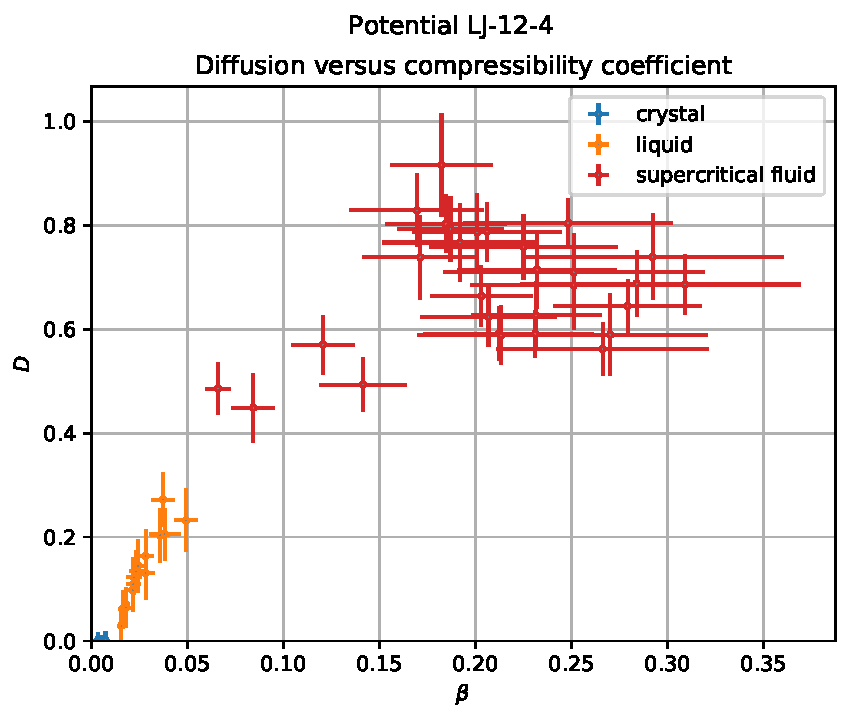
\includegraphics[width=\textwidth, keepaspectratio]{plot_diffusion_compress_Potential LJ-12-4_1}
\end{minipage}
%\hfill
\begin{minipage}[h]{0.45\linewidth}
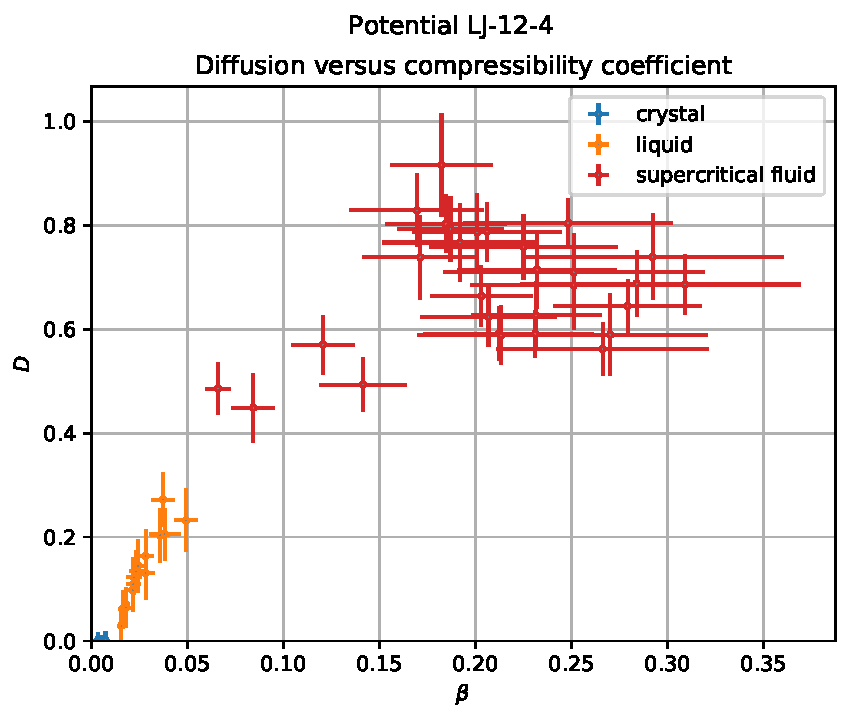
\includegraphics[width=\textwidth, keepaspectratio]{plot_diffusion_compress_Potential LJ-12-4_1}
\end{minipage}

%\vfill

\begin{minipage}[h]{0.45\linewidth}
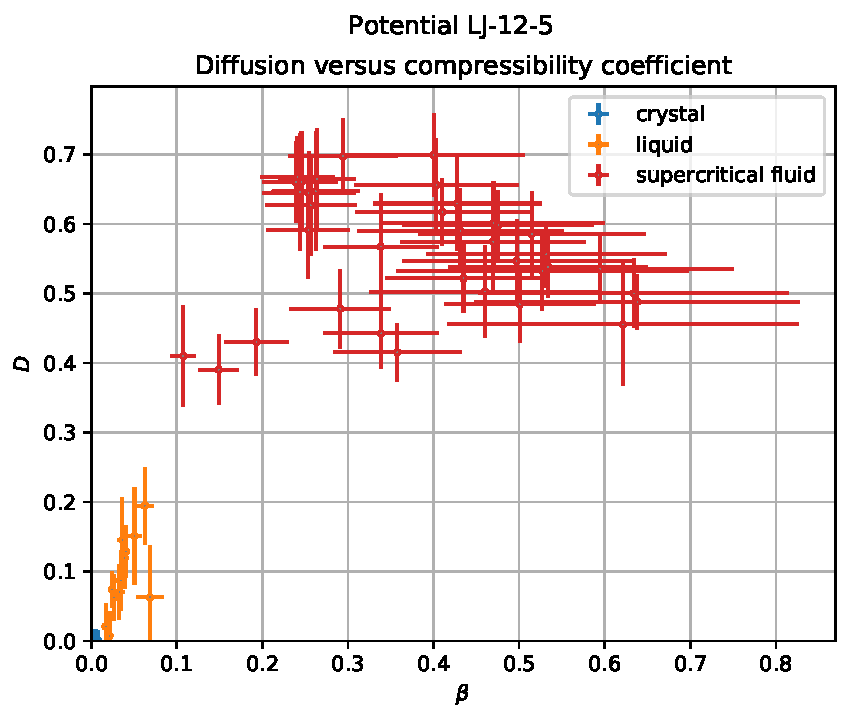
\includegraphics[width=\textwidth, keepaspectratio]{plot_diffusion_compress_Potential LJ-12-5_1}
\end{minipage}
%\hfill
\begin{minipage}[h]{0.45\linewidth}
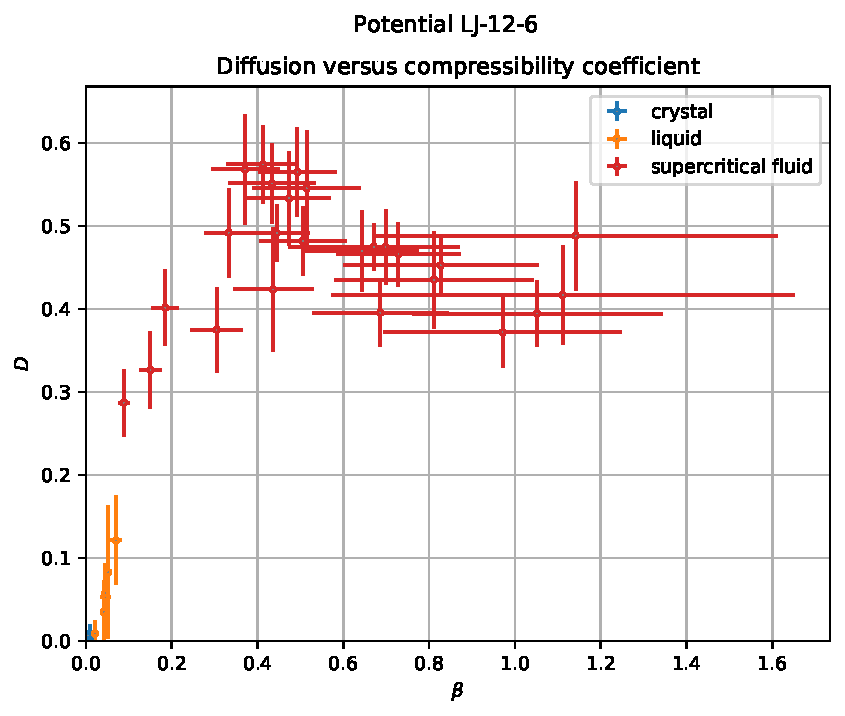
\includegraphics[width=\textwidth, keepaspectratio]{plot_diffusion_compress_Potential LJ-12-6_1}
\end{minipage}
\caption{Зависимость мобильности от сжимаемости. Не доделана!}
\label{ris21}
\end{center}
\end{figure}

Текст

Текст

\begin{figure}[htbp!]
\begin{center}
\begin{minipage}[h]{0.45\linewidth}
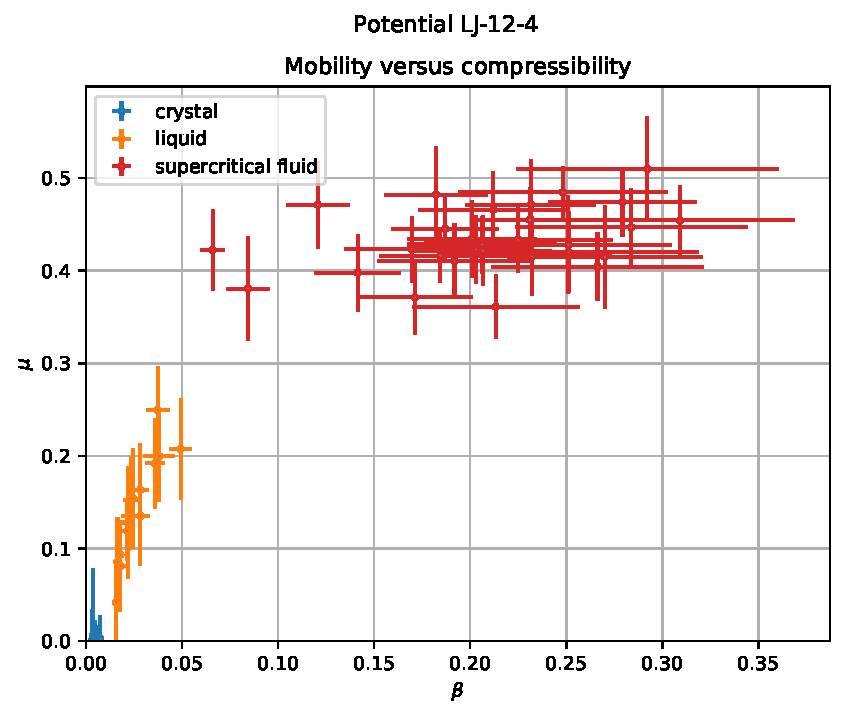
\includegraphics[width=\textwidth, keepaspectratio]{plot_compress_mobility_Potential LJ-12-4_1}
\end{minipage}
%\hfill
\begin{minipage}[h]{0.45\linewidth}
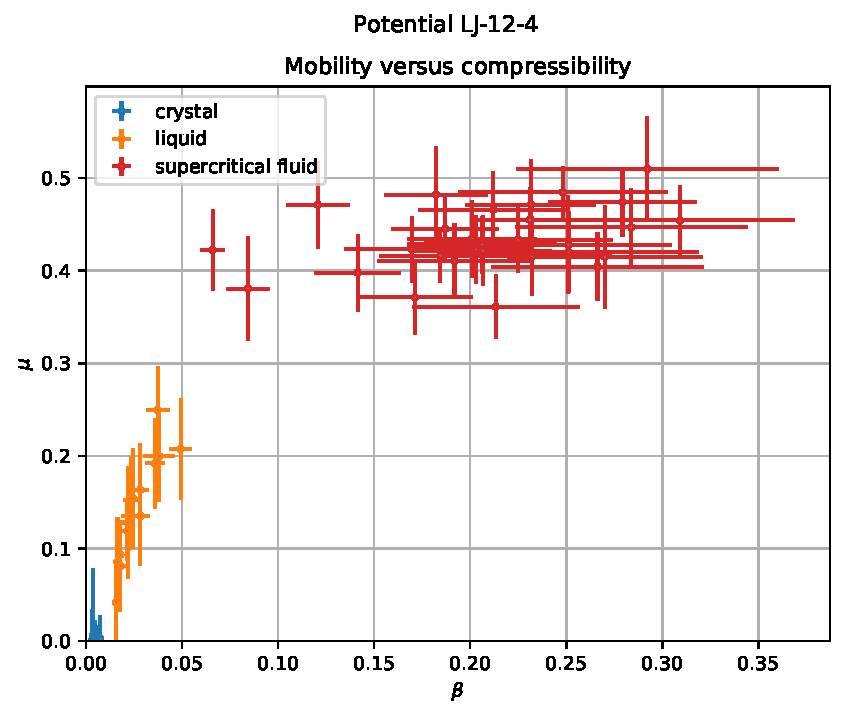
\includegraphics[width=\textwidth, keepaspectratio]{plot_compress_mobility_Potential LJ-12-4_1}
\end{minipage}

%\vfill

\begin{minipage}[h]{0.45\linewidth}
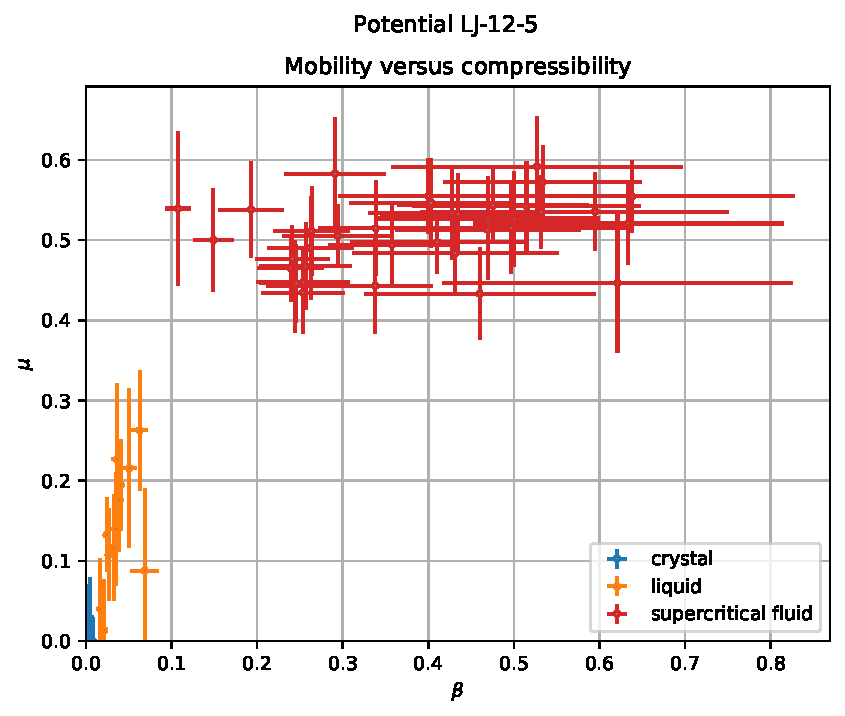
\includegraphics[width=\textwidth, keepaspectratio]{plot_compress_mobility_Potential LJ-12-5_1}
\end{minipage}
%\hfill
\begin{minipage}[h]{0.45\linewidth}
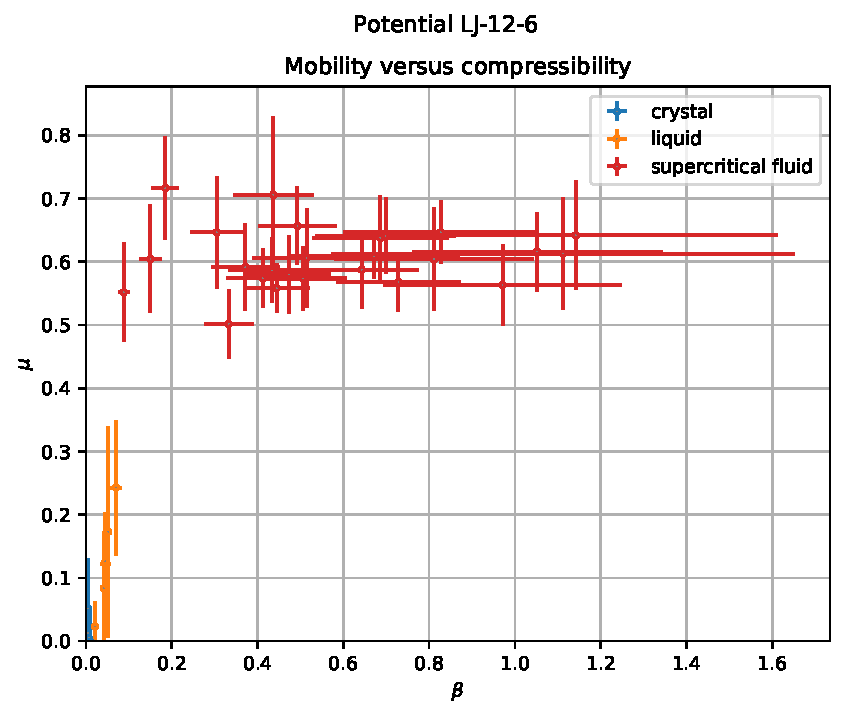
\includegraphics[width=\textwidth, keepaspectratio]{plot_compress_mobility_Potential LJ-12-6_1}
\end{minipage}
\caption{Зависимость мобильности от сжимаемости. Не доделана!}
\label{ris22}
\end{center}
\end{figure}

Текст

Текст

\begin{figure}[htbp!]
\begin{center}
\begin{minipage}[h]{0.45\linewidth}
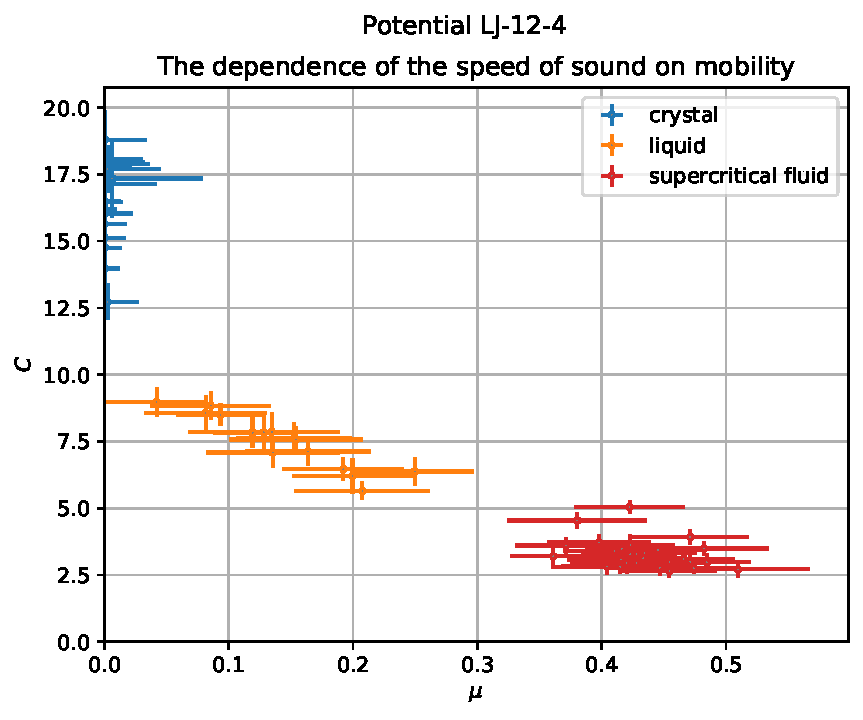
\includegraphics[width=\textwidth, keepaspectratio]{sound_speed_mobility_Potential LJ-12-4_1}
\end{minipage}
%\hfill
\begin{minipage}[h]{0.45\linewidth}
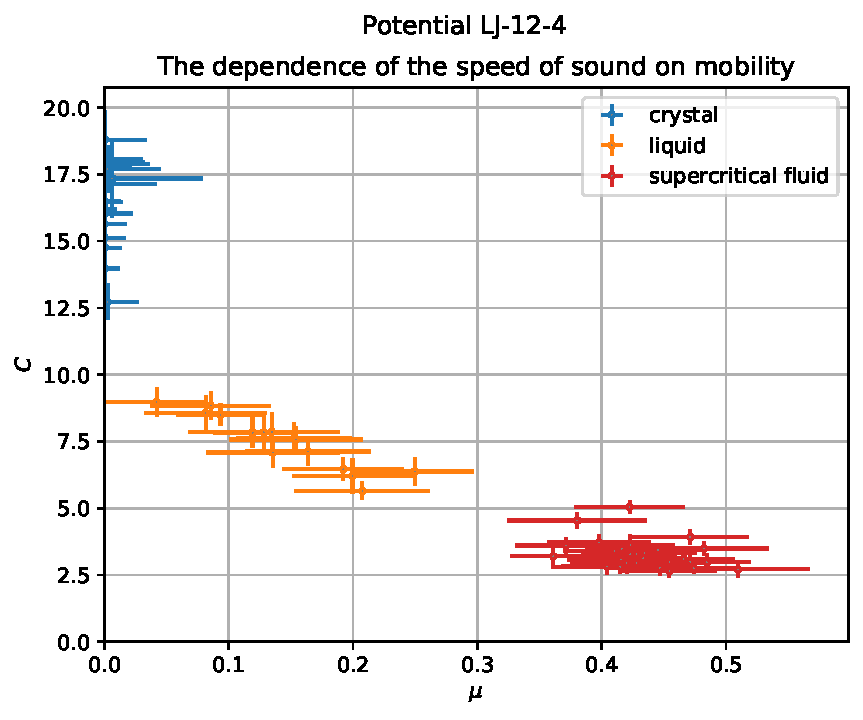
\includegraphics[width=\textwidth, keepaspectratio]{sound_speed_mobility_Potential LJ-12-4_1}
\end{minipage}

%\vfill

\begin{minipage}[h]{0.45\linewidth}
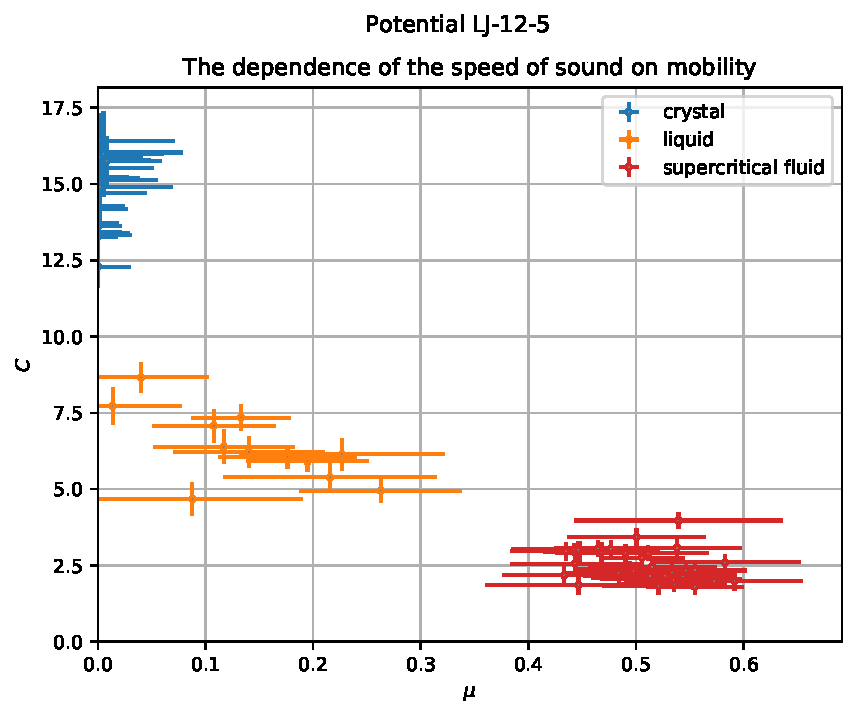
\includegraphics[width=\textwidth, keepaspectratio]{sound_speed_mobility_Potential LJ-12-5_1}
\end{minipage}
%\hfill
\begin{minipage}[h]{0.45\linewidth}
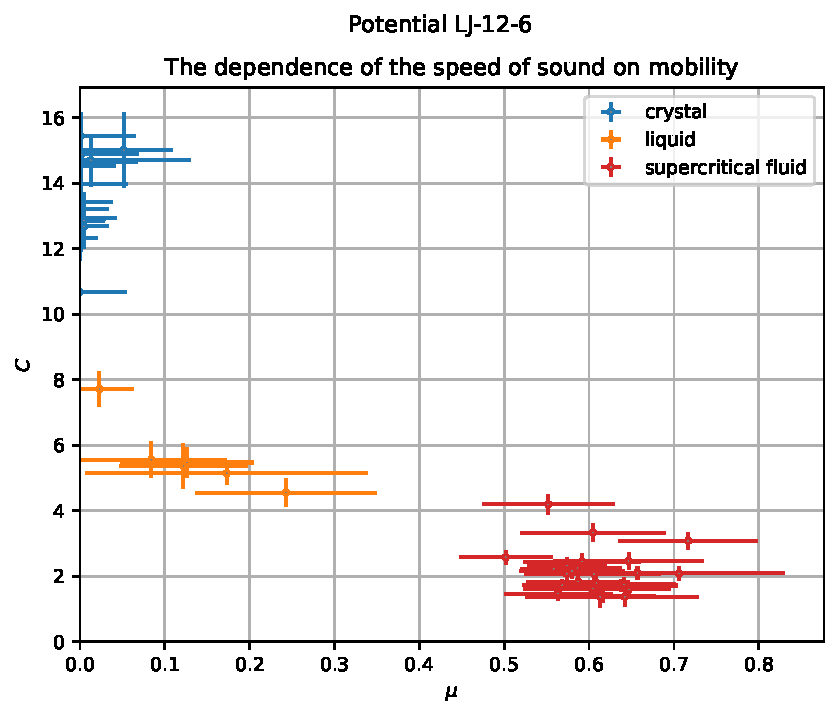
\includegraphics[width=\textwidth, keepaspectratio]{sound_speed_mobility_Potential LJ-12-6_1}
\end{minipage}
\caption{Зависимость мобильности от сжимаемости. Не доделана!}
\label{ris23}
\end{center}
\end{figure}

Текст

\section{Выводы главы}\label{C3_3}

Вывод